%
% Capítulo 3
%
\chapter{Architecture} \label{cap:architecture}

This chapter provides an overview of the system’s components and their interactions.
It outlines the capabilities of the project and presents the architecture, entities, and
implementation blueprint that have been designed and developed.

\section{Overview}

Figure ~\ref{fig:architecture} presents a diagram illustrating the main components of the system and their interactions. The system consists of a backend application (server-side) and a frontend application (client-side).
The backend comprises a collection of services, responsible for data processing and storage in a ElasticSearch database.
The frontend is composed of a web application, that facilitates user interaction. Communication between the frontend and the backend is achieved through a REST API, utilizing the HTTP protocol [24].

\begin{figure}[H]
	\begin{center}
		\resizebox{150mm}{!}{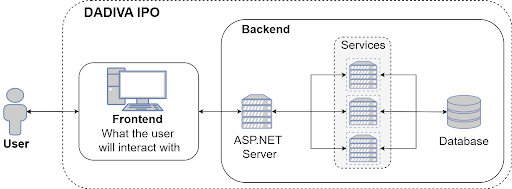
\includegraphics{./figures/Architecture.png}}
	\end{center}
	\caption{Application Architecture.}\label{fig:architecture}
\end{figure}

\section{Form Data Model}

The first approach to solve de dynamic form challenge was to use a data structure formed by main questions and sub-questions, example presented in Figure ~\ref{fig:old_form}, where a main question can only be answered with boolean values, and one of those values triggers the display of a sub-question which has a certain type of response, such as boolean, dropdown for known multiple answers, which needed an extra field, response range, to specify possible values, and text to accept user text input.


\begin{figure}[H]
	\begin{center}
		\resizebox{150mm}{!}{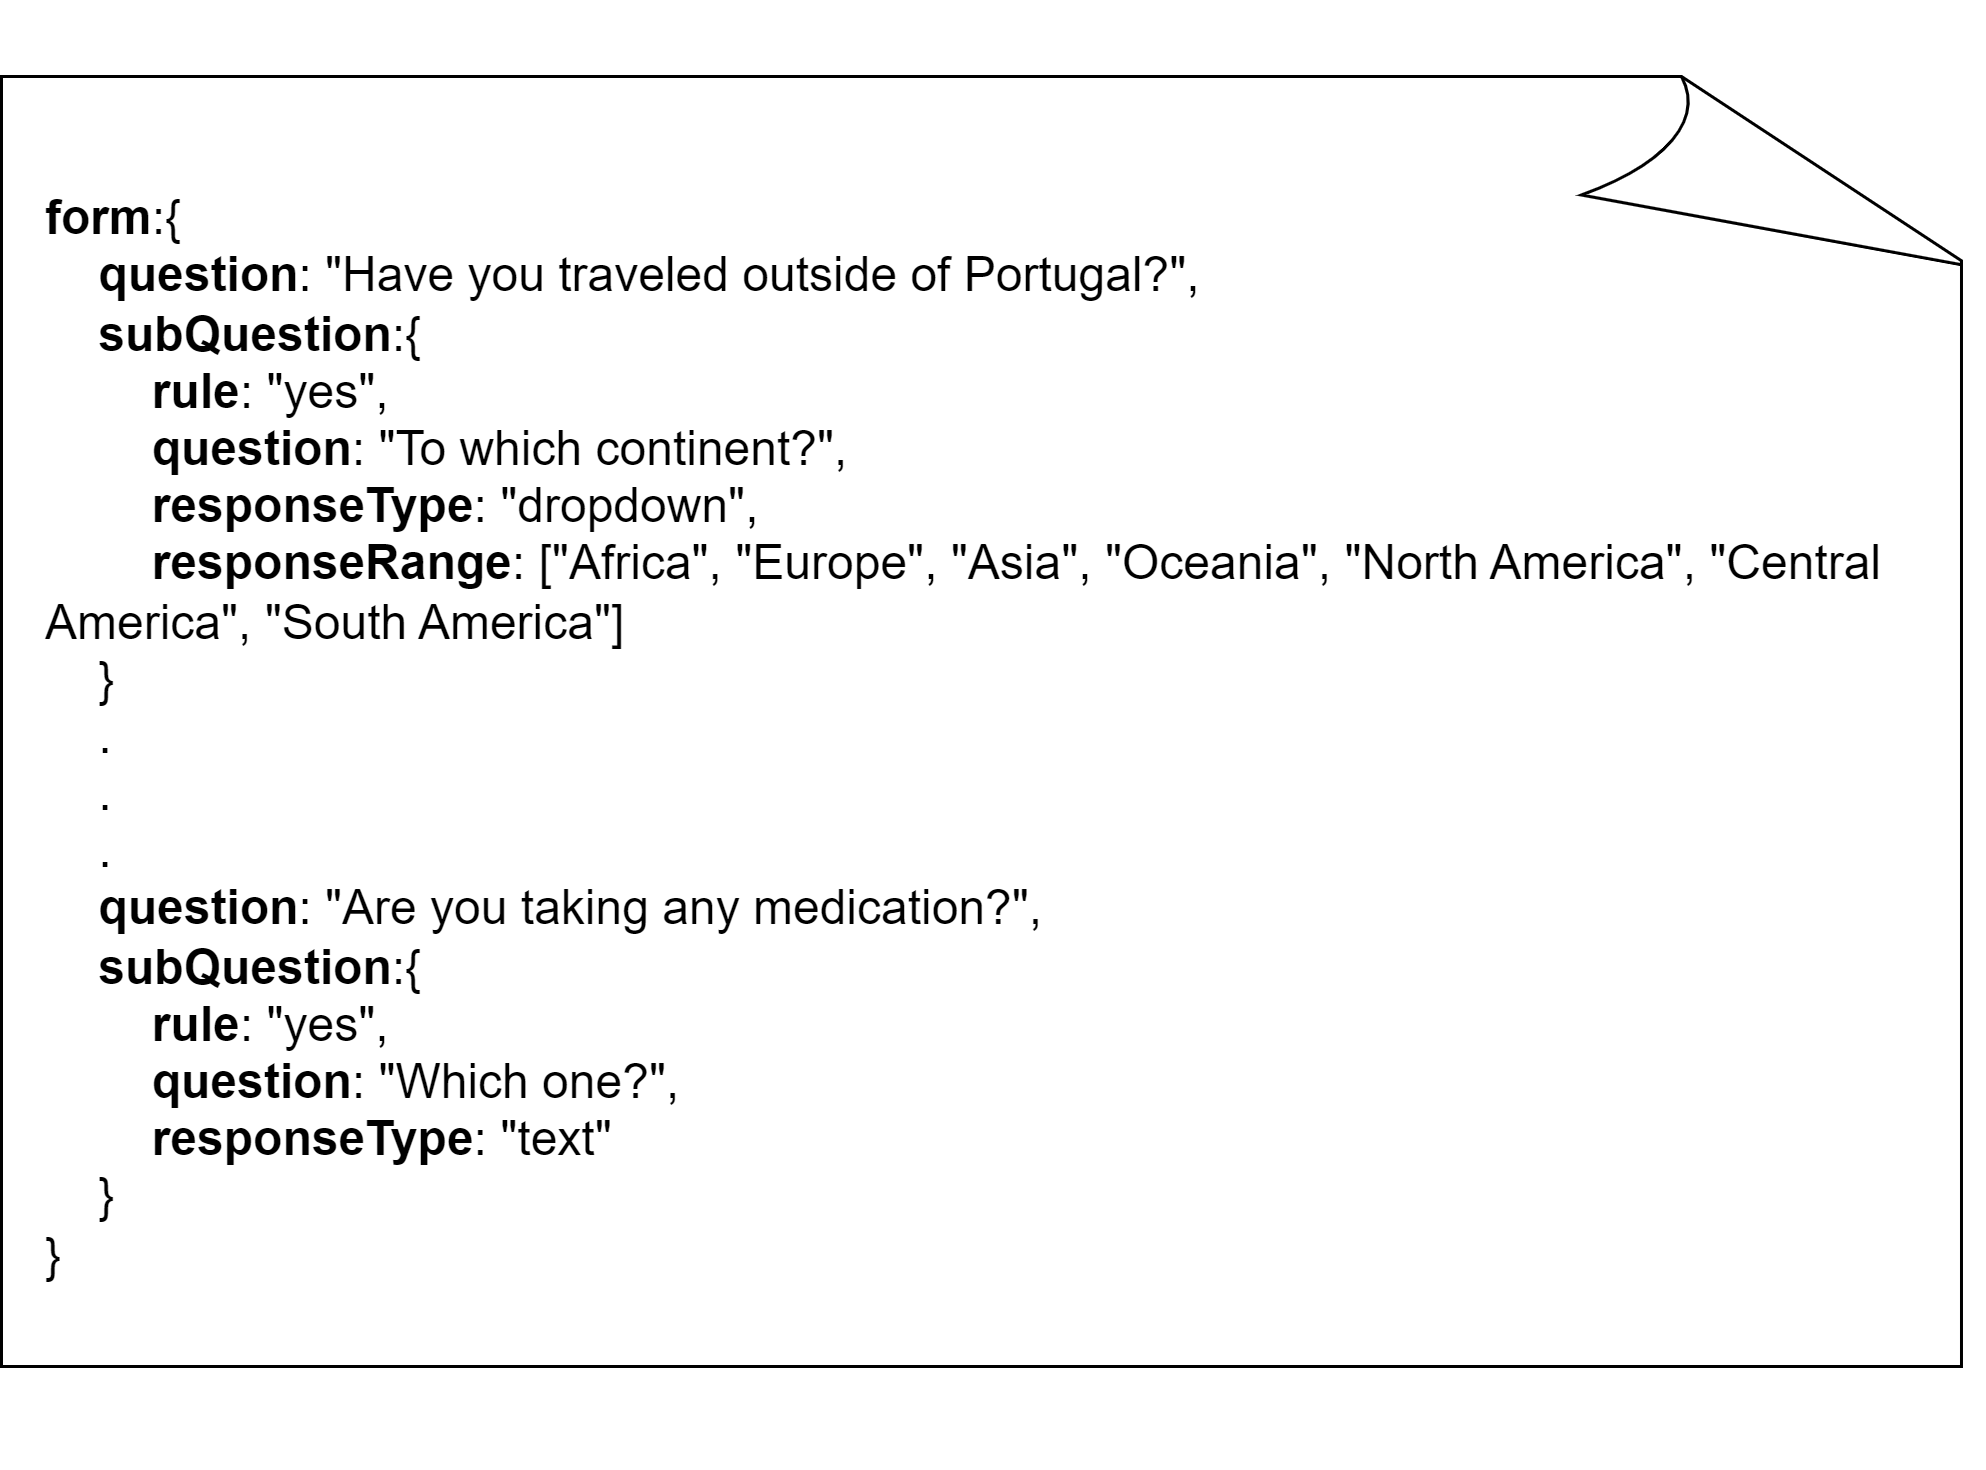
\includegraphics{./figures/oldForm.png}}
	\end{center}
	\caption{First Form Data Structure.}\label{fig:old_form}
\end{figure}

This approach has some drawbacks, such as the fact that it disables the possibility of supressing further questions hence not adhering to the principle of creating an adaptable solution, and mixes questions and rules in the sub-question.

Upon further discussion we settled on using a more complex data structure , exemplified in Figure ~\ref{fig:new_form}, composed by a list of questions and a list of rules.

Each question has an id, the text that composes it and the type of responses.

Each rule has a condition, which can be "any","all","not" and when any, all or none of the conditions are met an event is triggered, which can be to show os hide a question, the question's id that's being targeted by the event is supplied via the params field.


\begin{figure}[H]
	\begin{center}
		\resizebox{150mm}{!}{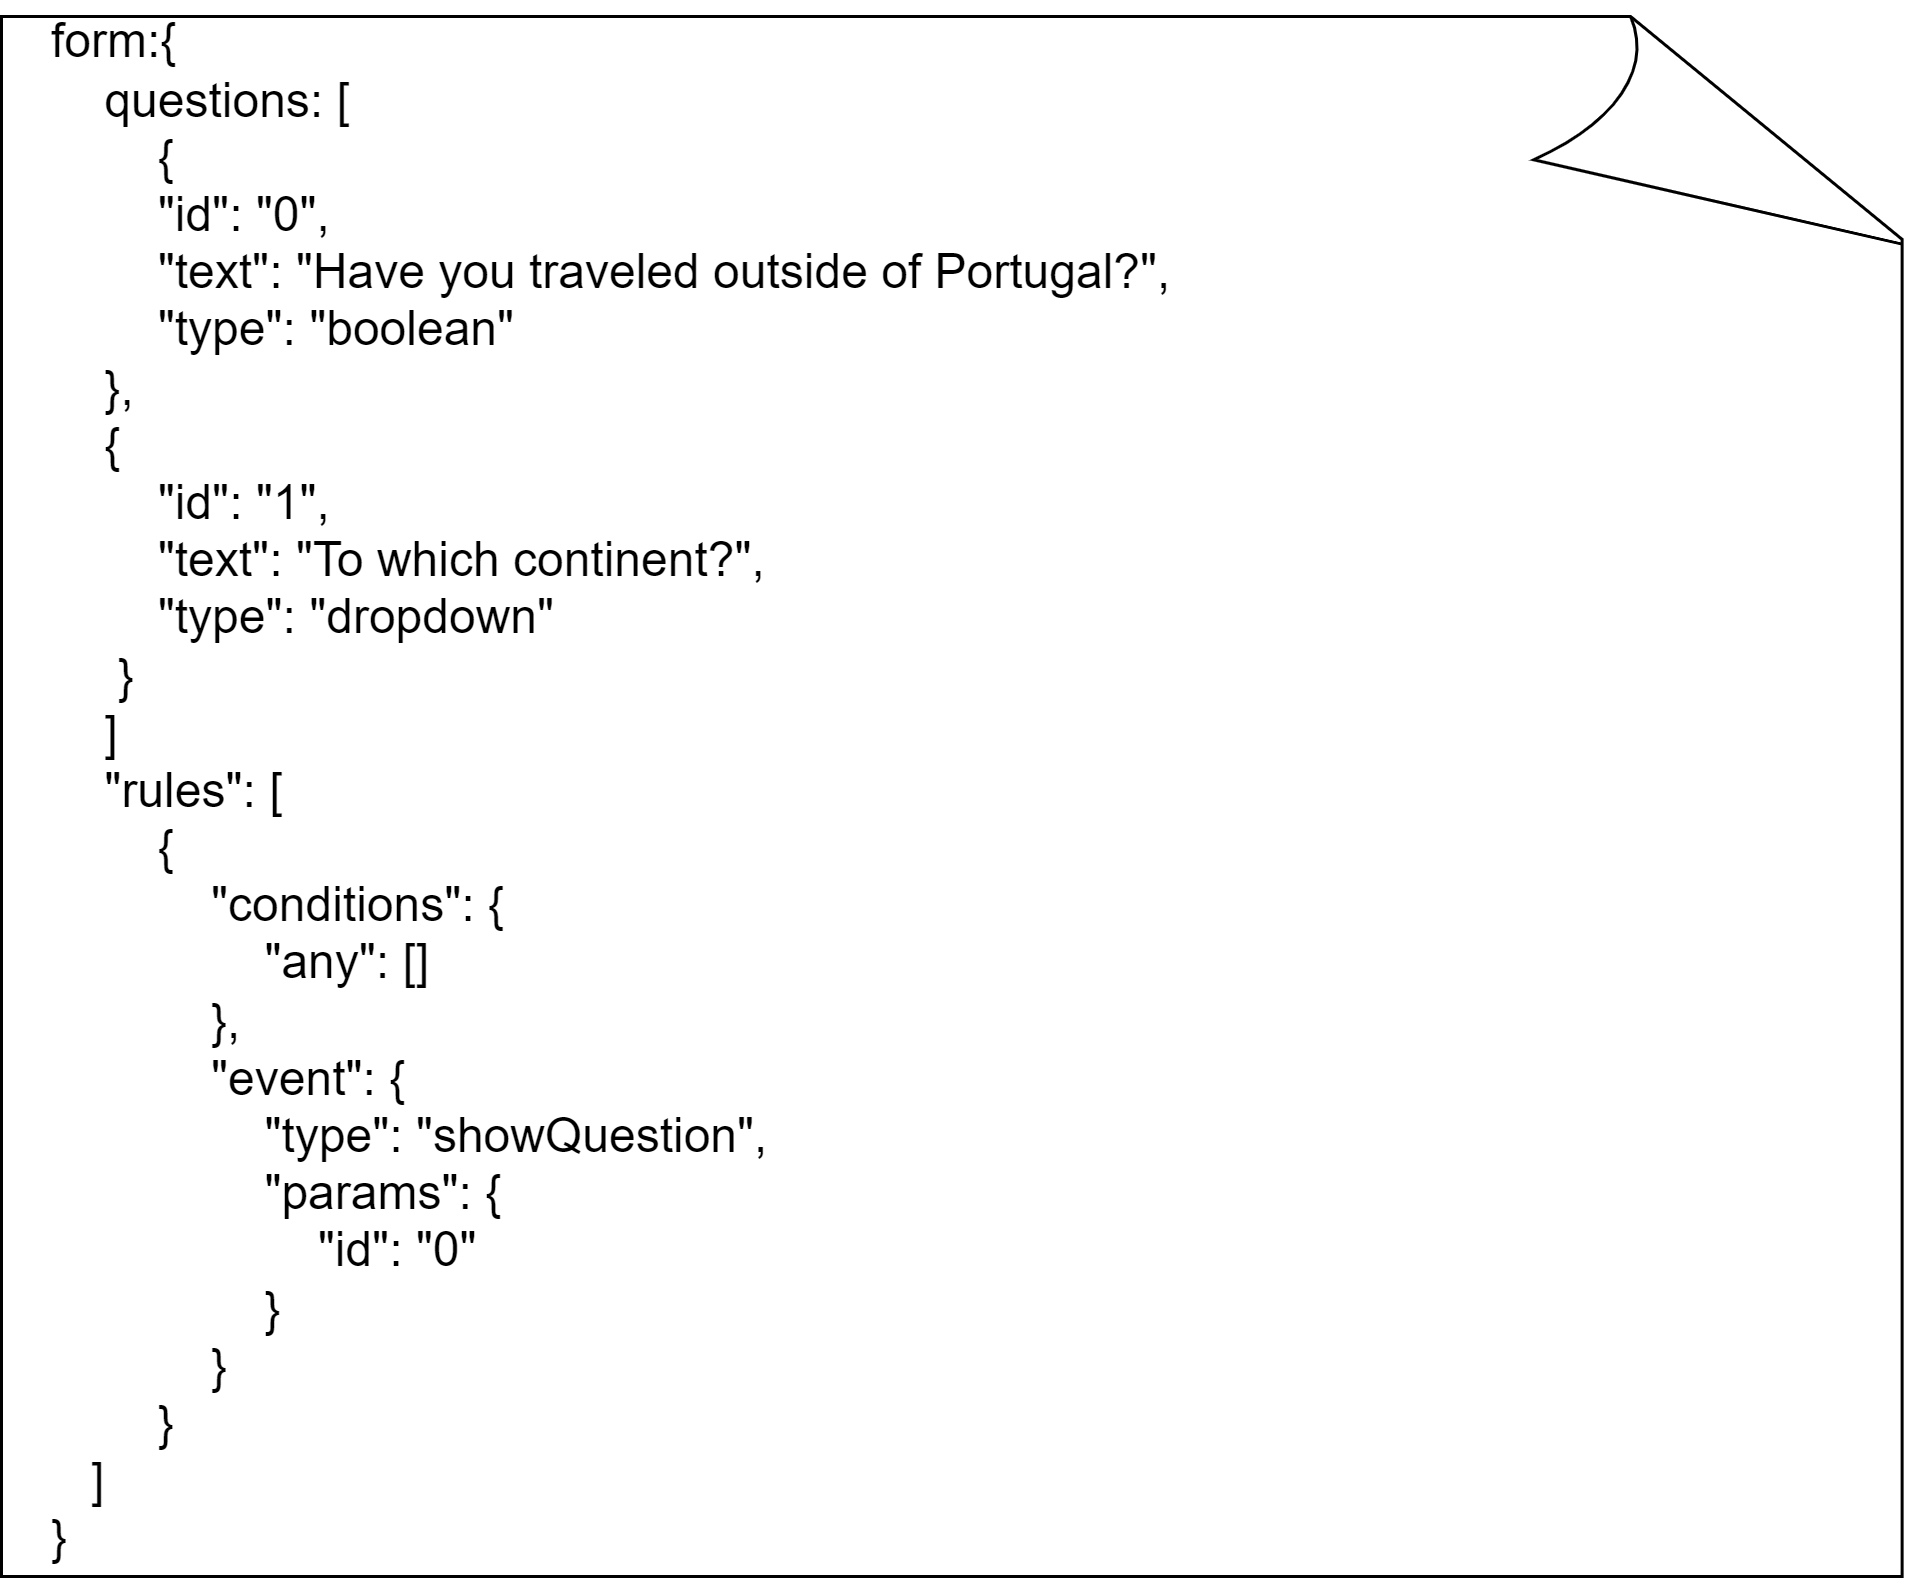
\includegraphics{./figures/newForm.png}}
	\end{center}
	\caption{Final Form Data Structure.}\label{fig:new_form}
\end{figure}


